\documentclass[../mcmpaper]{subfiles}
\begin{document}
	\section{Analysis of the Problem}
	\begin{figure}[h]
		\small
		\centering
		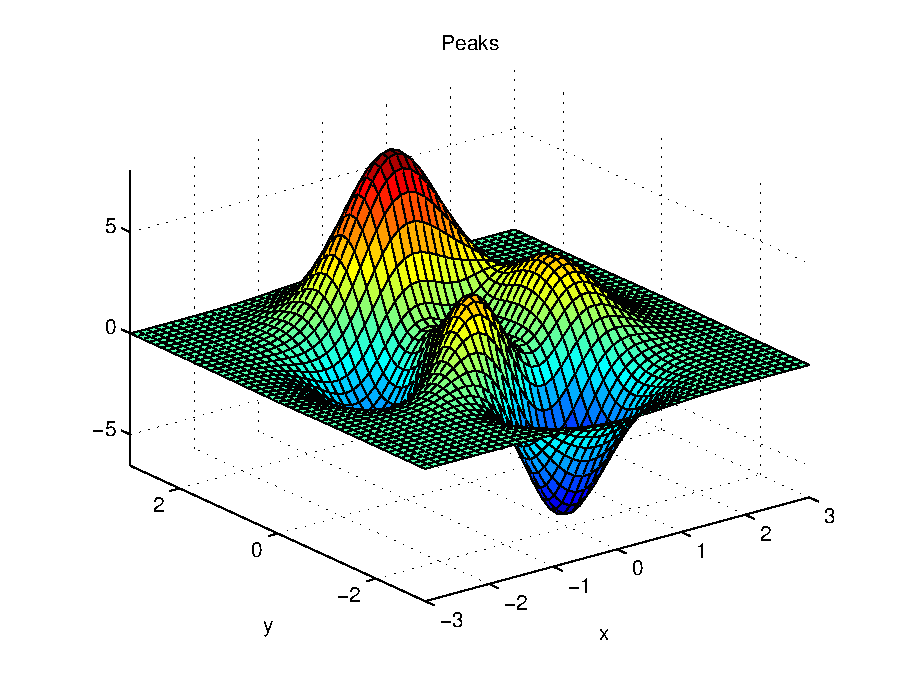
\includegraphics[width=12cm]{mcmthesis-aaa.eps}
		\caption{aa} \label{fig:aa}
	\end{figure}
	
	\lipsum[8] \eqref{aa}
	\begin{equation}
		a^2 \label{aa}
	\end{equation}
	
	\[
	\begin{pmatrix}{*{20}c}
		{a_{11} } & {a_{12} } & {a_{13} }  \\
		{a_{21} } & {a_{22} } & {a_{23} }  \\
		{a_{31} } & {a_{32} } & {a_{33} }  \\
	\end{pmatrix}
	= \frac{{Opposite}}{{Hypotenuse}}\cos ^{ - 1} \theta \arcsin \theta
	\]
	\lipsum[9]
	
	\[
	p_{j}=\begin{cases} 0,&\text{if $j$ is odd}\\
		r!\,(-1)^{j/2},&\text{if $j$ is even}
	\end{cases}
	\]
	
	\lipsum[10]
	
	\[
	\arcsin \theta  =
	\mathop{{\int\!\!\!\!\!\int\!\!\!\!\!\int}\mkern-31.2mu
		\bigodot}\limits_\varphi
	{\mathop {\lim }\limits_{x \to \infty } \frac{{n!}}{{r!\left( {n - r}
				\right)!}}} \eqno (1)
	\]
\end{document}
%%% Local Variables:
%%% mode: latex
%%% TeX-master: "../mcmpaper"
%%% End:
